%%%%%%%%%%%%%%%%%%%%%%%%%%%%%%%%%%%%%%%%%
% Short Sectioned Assignment
% LaTeX Template
% Version 1.0 (5/5/12)
%
% This template has been downloaded from:
% http://www.LaTeXTemplates.com
%
% Original author:
% Frits Wenneker (http://www.howtotex.com)
%
% License:
% CC BY-NC-SA 3.0 (http://creativecommons.org/licenses/by-nc-sa/3.0/)
%
%%%%%%%%%%%%%%%%%%%%%%%%%%%%%%%%%%%%%%%%%

%----------------------------------------------------------------------------------------
%	PACKAGES AND OTHER DOCUMENT CONFIGURATIONS
%----------------------------------------------------------------------------------------

\documentclass[paper=letter, fontsize=10pt]{scrartcl} % A4 paper and 11pt font size

\usepackage[T1]{fontenc} % Use 8-bit encoding that has 256 glyphs
\usepackage{fourier} % Use the Adobe Utopia font for the document - comment this line to return to the LaTeX default
\usepackage[english]{babel} % English language/hyphenation
\usepackage{amsmath,amsfonts,amsthm} % Math packages
\usepackage{graphicx}
\usepackage{caption}
\usepackage[titletoc,title]{appendix}
\usepackage{titlesec}
\usepackage{footnote}
\usepackage{sectsty} % Allows customizing section commands
\allsectionsfont{\centering \normalfont\scshape} % Make all sections centered, the default font and small caps

\makesavenoteenv{tabular}

\usepackage{fancyhdr} % Custom headers and footers
\pagestyle{fancyplain} % Makes all pages in the document conform to the custom headers and footers
\fancyhead{} % No page header - if you want one, create it in the same way as the footers below
\fancyfoot[L]{} % Empty left footer
\fancyfoot[C]{} % Empty center footer
\fancyfoot[R]{\thepage} % Page numbering for right footer
\renewcommand{\headrulewidth}{0pt} % Remove header underlines
\renewcommand{\footrulewidth}{0pt} % Remove footer underlines
\setlength{\headheight}{13.6pt} % Customize the height of the header

%\numberwithin{equation}{section} % Number equations within sections (i.e. 1.1, 1.2, 2.1, 2.2 instead of 1, 2, 3, 4)
%\numberwithin{figure}{section} % Number figures within sections (i.e. 1.1, 1.2, 2.1, 2.2 instead of 1, 2, 3, 4)
%\numberwithin{table}{section} % Number tables within sections (i.e. 1.1, 1.2, 2.1, 2.2 instead of 1, 2, 3, 4)

% \setlength\parindent{0pt} % Removes all indentation from paragraphs - comment this line for an assignment with lots of text

%----------------------------------------------------------------------------------------
%	TITLE SECTION
%----------------------------------------------------------------------------------------

\newcommand{\horrule}[1]{\rule{\linewidth}{#1}} % Create horizontal rule command with 1 argument of height

\title{	
\normalfont \normalsize 
\textsc{ME 552} \\ [25pt] % Your university, school and/or department name(s)
\horrule{0.5pt} \\[0.4cm] % Thin top horizontal rule
\huge Report for Lab 1: Calibration of Volumetric Flow Measurement Devices \\ % The assignment title
\horrule{2pt} \\[0.5cm] % Thick bottom horizontal rule
}

\author{Andrew Alferman} % Your name

\date{\normalsize\today} % Today's date or a custom date

\begin{document}

\iffalse
%THINGS HERE ARE THE OBJECTIVES TO HIT ON FROM THE LAB 1 FILE
To include in report:

Part 1: 	Plots of the calibration for both the orifice plates and the rotameters.

Part 2:	The value reported by the Isco-pumps as the independent variable and the calibrated flow rate as the dependent variable.

Part 3:	Plot data for MKS inputs to actual flow rates determined by Gilibrator.  Be sure to show uncertainty bars (design state uncertainty on the measured and dependent variables.


Questions to answer:

Part 1:	1) How does the discharge coefficient compare to that reported for the orifice plate?  Is the discharge coefficient constant for compressible and incompressible flow?
		2) Are compressibility effects a concern for the rotameter over the range that you studied? Justify your answer.

Part 2:	1) Are the values reported by the Isco-pumps appropriate to use, or does a calibration need to be applied to the values reported for the Isco-pumps.  Consider if values fall within the uncertainty bounds.

Part 3:	1) Discuss why the calibrated and MKS reported values are linearly related or not

\fi

\maketitle % Print the title

\section{Introduction}
\label{intro}
Three separate volumetric flow measurement experiments were conducted using a variety of common sensors and flow control equipment.  In the first experiment, air was directed through an orifice plate, a rotameter, and a dry test meter installed in series.  The orifice plate and rotameter were both calibrated using pressure data and measurements taken from the dry test meter.  The volumetric flow rate of water from an Isco-pump was calibrated in the second experiment using a calibrated scale and a stopwatch.  The volumetric flow rate of air through a MKS controller was measured in the third experiment using a bubble calibrator device.  The data obtained from the experiments was analyzed to determine the impact of compressibility effects and an uncertainty analysis was performed.  The objectives of these experiments were to familiarize the student with calibrating and using volumetric flow rate measurement equipment and to obtain flow rate data that will be used in a later experiment using a controlled flame.

\section{Methodology}
\subsection{Experiment Description}
In the first experiment, filtered shop air was directed through an orifice, a rotameter, and a dry test meter that were installed in series.  The flow rate was throttled using a valve in the rotameter to a predetermined value.  A data acquisition system was started and the pressure drop across the orifice was measured using pressure transducers located immediately upstream and downstream of the orifice.  Additionally, the temperature of the air was measured.  A stopwatch was started and the dry test meter dial was photographed.  After approximately four minutes, the dry test meter dial was photographed again.  The stopwatch was in the frame of each photograph, allowing the time in between photographs to be estimated to the nearest hundredth of a second.  By dividing the number of revolutions of the dry test meter dial by the time between the photograph, a flow rate was obtained.  The pressure measurements recorded by the data acquisition system and the information obtained from the dry test meter with the stopwatch were used to determine the orifice discharge coefficient and the rotameter calibration constant using equations included in appendix \ref{app:Method}.
\newline
\newline
The volumetric flow rate of water through an Isco-pump was measured in the second experiment using a calibrated scale and a stopwatch.  An empty container was placed on the scale and the pump outlet was positioned to discharge into the container.  After zeroing the scale with the container on it, the pump was started at the same time that a stopwatch was started.  After 90 seconds, the pump was stopped and the weight of the container with water was recorded.  The weight of the water divided by the stopwatch time provided a mass flow rate for the water, which could later be converted to a volumetric flow rate given the density of water.  The flow rate obtained from the Isco-pump was compared against the measured flow rate.
\newline
\newline
Air was directed through a small MKS thermal mass flow controller and a bubble calibrator device in the third experiment.  After starting the data acquisition system, the bubble calibrator was used to measure the flow rate.  The flow rate obtained from the MKS controller output was compared against the flow rate obtained from the bubble calibrator device.

\subsection{Equipment Used}
A list of all of the equipment used can be found in Appendix \ref{app:Equip}.

\subsection{Data Analysis}
The methodology and equations used to determine the discharge coefficients, calibration constants, and mass and volumetric flow rates is described in appendix \ref{app:Method}.

\section{Assumptions}
To make calibration of equipment possible, at least one measurement device in each experiment was assumed to be calibrated prior to collecting data.  These measurement devices were the pressure transducers and the dry test meter in the first experiment, the scale in the second experiment, and the bubble calibrator in the third experiment.
Information regarding the tolerance of each measurement device can be found in appendix \ref{app:Equip}
\newline
\newline
The assumed condition in which compressibility effects are significant is as follows:

\begin{equation}
\frac{P_1 - P_2}{P_1} \geq 0.1
\end{equation}

in which \(P_1\) is the upstream pressure and \(P_2\) is the downstream pressure, as measured by the pressure transducers.
\newline
\newline
The density of water was assumed to be 1000.0 \(\text{kg}/\text{m}^3\) and the \(c_p\) of water was assumed to be 4186 \(\text{J} / \text{kg} \cdot \text{K}\).  If needed, the density and \(c_p\) of air were varied in calculations based on experimental conditions, however an ideal gas constant of 287.05 \(\text{J} /\text{kg} \cdot \text{K}\) was used.
\newline
\newline
The compressibility factor Y of equation \ref{eq:1} of appendix \ref{app:Method} is assumed to be equal to one for the purpose of comparing the observed discharge coefficient to that reported by the manufacturer.  This assumption is a source of inaccuracy, however information regarding a more accurate compressibility factor was not readily available.

\section{Results}
A plot of the discharge coefficient times the compressibility factor of the orifice can be found in figure \ref{plot:exp1}.  The large degree of uncertainty attributed to the lower flow rates of the graph is due to the relatively large tolerance of the pressure transducers used in the experiment.  To demonstrate the impact of the 0.25 psi pressure transducer tolerance, the differential pressure across the orifice was less than the pressure transducer tolerance with an observed flow rate of 1.2 scfm, and the pressure transducers in fact measured a greater pressure downstream of the orifice than the pressure upstream of the orifice.  The uncertainty improved greatly at higher flow rates as the differential pressure across the orifice increased to values greater than the tolerance of the pressure transducers.

\begin{figure}[!h]\label{plot:exp1}
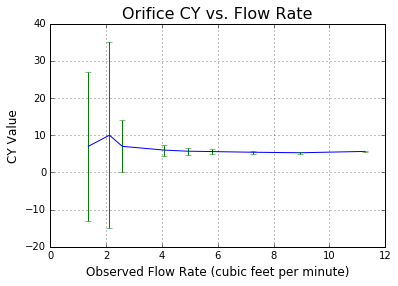
\includegraphics[scale=0.6]{Lab1FigureCY}
\centering
\end{figure}

The discharge coefficient of the orifice was found to have a value of approximately 5.5 at most flow rates.  This value is greater than the value reported by the manufacturer, which was calculated to be approximately 0.80 using the equation \(C_v = 38 A C_d\), where \(C_v\) was the value of 0.37 reported by the manufacturer, and A is the area of the opening of the orifice.  It cannot be determined if the discharge coefficient is constant for compressible and incompressible flows because no information regarding the compressibility factor Y is available.
\newline
\newline
Compressibility effects were a significant concern for the rotameter, as could be seen in figure \ref{plot:exp1A}.  The plot shows that as the flow rate increased, the rotameter increasingly underestimated the flow rate.

\begin{figure}[!h]
  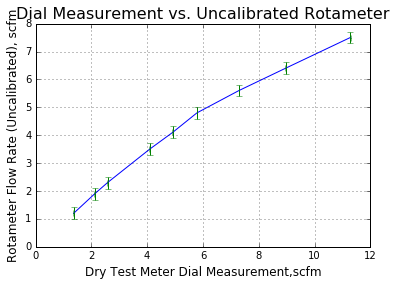
\includegraphics[scale=0.6]{Lab1FigureUncalRot} 
  \centering
  \label{plot:exp1A}
\end{figure}

After adding a correction factor to the rotameter flow rate (and thus calibrating the rotameter), a much better correlation could be derived.  Figure \ref{plot:exp1B} shows the calibrated rotameter values.  Note that there are error bars in both directions, however the error from the dry test meter is too small to be seen in this graph (tolerance of 0.01 scfm).

\begin{figure}[!h]
  \label{plot:exp1B}
  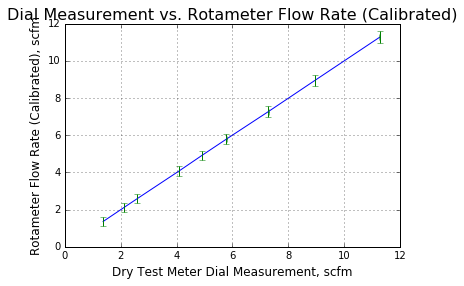
\includegraphics[scale=0.6]{Lab1FigureRot} 
  \centering
\end{figure}

Figure \ref{plot:exp2} is a graph of the flow rate value reported by the Isco-pump versus the measured flow rate.  As seen in the graph, the values match very closely.  There may be a need in some experiments to obtain a more precise value for the flow rate of a fluid, however the value reported by the Isco-pump is generally very good and would not require further calibration.  The reported values fell within the uncertainty bounds.

\begin{figure}[!h]
  \label{plot:exp2}
  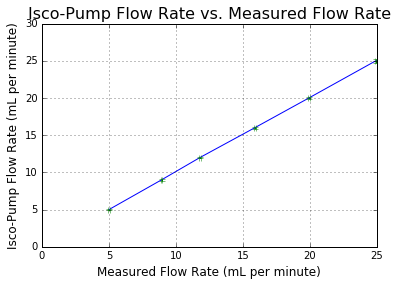
\includegraphics[scale=0.6]{Lab1FigureScale}
  \centering
\end{figure}

The plot shown in figure \ref{plot:exp3} below shows that the calibrated and MKS reported values are linearly related.  As the flow rate increases, the measured flow rate using the Gilibrator increases at a slightly higher rate, forming a linear relationship.

\begin{figure}
  \label{plot:exp3}
  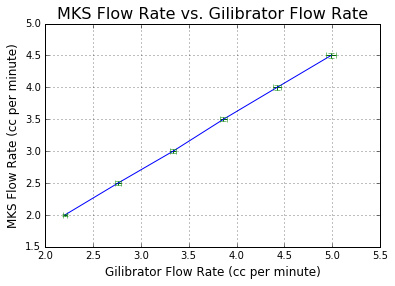
\includegraphics[scale=0.6]{Lab1FigureGili}
  \centering
\end{figure}

\section{Conclusion}
It was found through several experiments that the instruments used to measure flow rate need to be carefully selected to obtain accurate results.  For example, orifice flow meters using pressure transducers may give inaccurate results at low volumetric flow rates, while measurements from rotameters in high volumetric flow conditions need to be carefully examined to determine if the effects of compressible flow have been taken into account.  Every instrument used in this lab has advantages and disadvantages that need to be carefully considered.

\clearpage
\begin{appendices}
\setcounter{equation}{0}
% "INCLUDE IN THE APPENDIX DOCUMENTATION ABOUT HOW THE DESIGN STAGE UNCERTAINTY WAS DETERMINED, YOUR UNCERTAINTY TREES, AND ANYTHING THAT IS NEEDED TO SUPPORT YOUR DISCUSSION."
\section{Equipment Tolerances}\label{app:Equip}

\begin{table}[h]
\begin{center}
\begin{tabular}{ | c  c  c |}
 \hline
 Instrument & Model & Tolerance \\
 \hline\hline
 Orifice & O'Keefe Type H & See Table \ref{tab:orif} \\
 \hline
 Rotameter & Omega FL4611-V & +/- 2.5\% of Full Scale (0.2125 scfm)\\
 \hline
 Pressure Transducer & Omega PX309 & +/- 0.25\% Full Scale (.25 psi) \\
 \hline
 Thermocouple & Type K & +/- \(2.2^\circ\)C \\
 \hline
 Dry Test Meter & Singer DTM-200\footnote{The American Meter division of Singer was acquired through a series of transactions by Elster American Meter, therefore specifications on the Elster American Meter DTM-200 are assumed to be identical to the Singer DTM-200.} & +/- 0.01 standard cubic foot \\
 \hline
 Pump & Isco-pump Series D & +/- 0.1\% \\
 \hline
 Scale & AND FX-6000 & +/- 0.1 gram \\
 \hline
 Bubble Calibrator & Gilian Gilibrator D800268 & +/- 1\% of reading accuracy \\
 \hline
 Thermal Flow Controller & MKS GM50A & +/- 1\% of set point \\
 \hline
\end{tabular}
\end{center}
\caption{Equipment Used}\label{tab:tol}
\end{table}

\begin{table}[h]
\begin{center}
\begin{tabular}{ | c  c  c |}
 \hline
 Measurement & Nominal Value & Tolerance \\
 \hline
 Orifice Diameter & 0.1248 inch & +/- 0.0004472 inch \\
 \hline
 Upstream Diameter & 0.3105 inch & +/- 0.0009617 inch \\
 \hline
\end{tabular}
\end{center}
\caption{Orifice Dimensions}\label{tab:orif}
\end{table}

\clearpage

\section{Uncertainty Analysis}\label{app:Unc}
\subsection{Methodology}\label{app:Method}
An uncertainty analysis was conducted using the Kline McClintock method.  The uncertainty values were computed numerically in Python using the attached source code, however a depiction of how the Kline McClintock method worked in each phase of this lab is included in appendix \ref{app:Tree}.  Partial derivatives of each equation were taken until a tolerance from the manufacturer could be used.  In the case of the orifice, the openings were measured using calipers to obtain a more exact value.
\newline
\newline
The equation governing the subsonic volumetric flow rate through an orifice is as follows:

\begin{equation}\label{eq:1}
Q = C E A Y \sqrt{\frac{2 \Delta P}{\rho_1}}
\end{equation}

in which Q is the volumetric flow rate, C is the orifice discharge coefficient, A is the area of the orifice opening, Y is a compressibility constant, \(\Delta P\) is the pressure difference across the orifice, \(\rho_1\) is the density of the fluid upstream of the orifice (air in this case).  E is defined as follows:
\begin{equation}\label{eq:2}
E =  \frac{1}{\sqrt{1 - (\frac{A_0}{A_1})^2}}
\end{equation}

in which \(A_0\) and \(A_1\) are the area of the orifice opening and the area of the upstream piping, respectively.  The orifice in the first experiment is calibrated by solving for C in equation \ref{eq:1} of this appendix.  
\newline

%If it is instead found that choked flow conditions exist (i.e. the flow is sonic), the mass flow rate through the orifice is calculated using the following equation:
%
%\begin{equation}\label{eq:3}
%\dot{m}_{choked} = C \frac{P_0 A_1}{\sqrt{R T_0}}\sqrt{\frac{2k}{k+1}\Bigg(\frac{2}{k+1}\Bigg)^\frac{2}{k+1}}
%\end{equation}
%
%in which \(\dot{m}_{choked}\) is the mass flow rate of the fluid, \textit{k} is the ratio of specific heats upstream and downstream of the orifice. % ADD THE OTHER VARIABLES AS NEED BE

The equation governing the relationship between the actual flow rate through a rotameter and the observed flow rate through a rotameter is as follows:
\begin{equation}\label{eq:4}
Q_{actual} = C(P_{downstream}) Q_{observed}
\end{equation}

in which \(Q_{actual}\) is the actual volumetric flow rate, \(Q_{observed}\) is the observed volumetric flow rate, and C is a calibration constant that is a function of the downstream pressure, \(P_{downstream}\).

\subsection{Tree Diagram}\label{app:Tree}
A tree diagram for the orifice calibration has been attached.  Tree diagrams were not constructed for the other steps of this lab due to the simplicity of all of the subsequent calculations (no uncertainty values were affected by more than one or two variables, and partial derivatives were readily obtained).

\end{appendices}
\end{document}